\documentclass[oneside,reqno]{amsart}
\usepackage{amsthm}
\usepackage{dsfont}
\setlength{\textwidth}{\paperwidth}\addtolength{\textwidth}{-2in}\calclayout
\usepackage[utf8]{inputenc}
\usepackage{tikz}
\usepackage{minted}
\newminted{python3}{frame=lines}
\usepackage{booktabs}
\usepackage{enumitem}

\DeclareMathOperator{\E}{E}
\DeclareMathOperator{\var}{var}
\DeclareMathOperator{\cov}{cov}
\DeclareMathOperator{\corr}{corr}
\DeclareMathOperator{\tr}{tr}
\let\vec\relax\DeclareMathOperator{\vec}{vec}
\newcommand{\eps}{\varepsilon}

\theoremstyle{definition}
\newtheorem{prob}{Problem}
\renewcommand*{\proofname}{Solution}
\setlist[enumerate]{label={(\roman*)}}

\title{ECON 706: Problem Set 3}
\author{Daniel Pfeffer}
\date{\today}
%------------------------------------------------------------------------------
\begin{document}
\maketitle

\begin{prob}
Write a program which takes as inputs 2 uniformly distributed random variables and uses the Box-Muller approach to obtain 2 standard normally distributed random variables.
\end{prob}

\begin{proof}
The function \mintinline{python3}{box_muller} expects two uniform random variables of arbitrary size and generates realizations of two standard normal random variables using the Box-Muller approach.
\begin{python3code}
import numpy as np
import matplotlib.pyplot as plt

def box_muller(u1, u2):
    """u1, u2 are uniform random variables of size T
    Returns two N(0,1) random variables of size T"""
    z1 = np.sqrt(-2*np.log(1-u1))*np.cos(2*np.pi*u2)
    z2 = np.sqrt(-2*np.log(1-u1))*np.sin(2*np.pi*u2)
    return np.array([z1, z2])
\end{python3code}
\end{proof}

\begin{prob}
Consider the following 2-variable VAR(1):
\[
	y_t = \Phi y_{t-1} + \eps_t, 
	\qquad \eps_t \sim N(0, \Sigma),
\]
where $y_t = (y_{1t}, y_{2t})'$, $\eps_t = (\eps_{1t}, \eps_{2t})'$, 
\[
	\Phi = \begin{pmatrix}
		0.6 & 0 \\
		0.9 & 0.3 
	\end{pmatrix},
\]
and where $\Sigma$ is such that $\var(y_{1t}) = 2$, $\var(y_{2t}) = 8$ and  $\corr(y_{1t}, y_{2t}) = 0.5$. For $T=1000$, use your program from exercise 1 to simulate $\{y_{1t}, y_{2t}\}_{t=1}^T$. Draw $y_0$ from the unconditional distribution of $y_t$.
\end{prob}

\begin{proof}
To fully specify the covariance matrix, notice that
\[
	\cov(y_{1t}, y_{2t}) =\corr(y_{1t}, y_{2t}) \sqrt{\var(y_{1t})\var(y_{2t})} = 0.5 \sqrt{2 \cdot 8} = 2.
\]
which implies that
\[
	\Sigma = \begin{pmatrix}
			2 & 2 \\
			2 & 8
	\end{pmatrix},
\] 
Then generate two $U([0,1])$ random variables of size $T=1000$ and call \mintinline{python3}{box_muller} to simulate $x = (x_1, x_2)' \sim N(0,I)$.  Recall that since every covariance matrix $\Sigma$ is positive semidefinite, there exists a Cholesky factorization $\Sigma = PP'$, where $P$ is a lower triangular matrix. So $\eps_t = P x \sim N(0, \Sigma)$. Note that this also gives the initial draw for $y_0$ from the unconditional distribution of $y_t$. Finally, applying the autoregressive operator $\Phi$ to innovations $\eps_t$ along with the initial condition given by $y_0$ generates samples from the desired system. The following code implements this VAR(1) simulation.

\begin{python3code}
# Initialize VAR(1) system parameters
Phi = [[.6, 0], [.3, .9]]
Sigma= [[2, 2], [2, 8]]

# Generate two U([0,1]) random varialbes 
np.random.seed(42)
T = 1000
u1, u2 = np.random.rand(T), np.random.rand(T)

# Simulate N(0,I) random vector 
iid_innov = box_muller(u1, u2)

# Generate innovations via Cholesky factorization  
L = np.linalg.cholesky(Sigma)
eps = np.dot(L, iid_innov)
eps1, eps2 = eps[0], eps[1]

# Allocate memory for y1 and y2 series 
y1, y2 = np.empty_like(eps1), np.empty_like(eps2)

# Draw y0 from unconditional distribution 
y1[0], y2[0] = eps1[0], eps2[0]

# Simulate y1 and y2 series  
for t in range(1, T):
    y1[t] = Phi[0][0]*y1[t-1] + eps1[t]
    y2[t] = Phi[1][0]*y1[t-1] + Phi[1][0]*y2[t-1] + eps2[t]
\end{python3code}
\end{proof}


\begin{prob}
Estimate the univariate spectral density function of $y_{1t}$ using the following approaches.
\begin{itemize}
\item
Take $\hat f(\omega) = (2\pi)^{-1} \sum_{\tau=-(T-1)}^{T-1} \hat \gamma(\tau) e^{-i \omega \tau}$, where $\hat \gamma$ are the sample autocovariances. 
\item
Use a uniform lag window with truncation lag of 10.
\item
Fit an AR($p$) model for $y_{1t}$ using a simple regression, where $p$ is chosen based on model selection criteria, and compute the spectral density function of your estimated model.
\end{itemize}
Plot and comment on the resulting estimated spectral densities.
\end{prob}


\begin{proof}
The sample spectral density computed by first estimating the periodogram 
\[
	I(\omega) = \frac{1}{T} \left| \sum_{t=0}^{T-1} y_t e^{2\pi i (\omega/T)t} \right|^2,
\]
and then scaling the resulting values by $4\pi$ to obtain
\[
	\hat f(\omega) =  \frac{1}{4\pi} I(\omega),
\]
which is equivalent to computing the sample autocovariance and taking its Fourier transform. This estimation procedure is implemented in the function \mintinline{python3}{sample_sdf}. The function \mintinline{python3}{unif_window} estimates the spectral density function by applying a uniform window with a truncation lag of 10 to the sample spectral density.  The function \mintinline{python3}{ar_sdf} fits an AR($p$) model to a vector of times series where the order $p$ is determined by the BIC and then the spectral density is then estimated using 
\[
	\hat f(\omega) = \frac{\hat\sigma^2}{2\pi} \left| \frac{1}{\phi(e^{i\omega})} \right|^2 
\]
where $\phi(z)$ is the autoregressive polynomial determined by the BIC, and $\hat \sigma^2$ is the sample variance.  

\begin{python3code}
def sample_sdf(y):
    """y is an array of time domain data 
    Returns w, the frequencies and f_y, the sample spectral density"""
    T = len(y)
    from numpy.fft import fft
    f_y = np.abs(fft(y))**2/T
    w = 2*np.pi*np.arange(T)/T
    w, f_y = w[:int(T/2)+1], f_y[:int(T/2)+1]
    return w, f_y/(4*np.pi)

def unif_window(f, trunc_lag=10):
    """f is the sample spectral density
    Return the uniform lag window sample spectral density"""
    j = int(trunc_lag/2)
    fb = f[:j]
    ft = f[-j:]
    s = np.concatenate((fb[::-1], f, ft[::-1]))
    window = np.ones(trunc_lag)
    return np.convolve(window/window.sum(), s, mode='valid')

def ar_sdf(y, max_lag=15, i_c='bic', cst='n'):
    """y is an array of time domain data 
    Returns w, the frequencies and ar_sdf, the ar sample spectral density"""
    from statsmodels.tsa.ar_model import ar_select_order
    sel = ar_select_order(y, maxlag=max_lag, ic=i_c, trend=cst)
    res = sel.model.fit()
    ar_poly = np.insert(-res.params, 0, 1)
    from scipy.signal import freqz
    w, b_fft = freqz(b=1, a=ar_poly, worN=int(len(y)/2)+1)
    ar_sdf = res.sigma2*np.abs(b_fft)**2/(4*np.pi)
    return w, ar_sdf

# Sample, Uniform lag window, and  autoregressive, SDFs for y1
w_y1, f_y1 = sample_sdf(y1)
w_y1_unif, f_y1_unif = unif_window(f_y1)
ar_freq_y1, b_fft_y1 = ar_sdf(y1)

# Plot results
plt.figure(figsize=(12,4))

plt.subplot(131)
plt.plot(w_y1, f_y1)
plt.title('Sample Spectral Density')

plt.subplot(132)
plt.plot(w_y1, f_y1_unif[1:])
plt.title('Uniform Window Spectral Density')

plt.subplot(133)
plt.plot(ar_freq_y1, ar_sdf_y1)
plt.title('AR Spectral Density')

plt.tight_layout()
plt.show()
\end{python3code}    

We make function calls on the simulated $y_{1t}$ process to estimate its spectral density according to these three alternative methods. Figure \ref{q3-fig} shows the plots of the resulting nonparametric sample spectral density estimates. The top graph shows the sample spectral density. Although it vaguely captures what Granger called the ``typical spectral shape'' associated with an AR(1) with $\phi > 0$, is a substandard estimate. In other words, although appears somewhat unbiased, the resulting figure displays clear evidence of inconsistency that can be seen in the highly fluctuating values on the $y$-axis. The second graph shows the uniform window with a truncation lag of 10 sample spectral density. This estimate smoothed out much of this inconsistency, as can be seen by noting the change in the values on the $y$-axis. The third plot shows the autoregressive spectral density estimate. The BIC made the correct model specification, as expected and the conditional maximum likelihood parameter estimate is 0.62, which differs from the ``true'' parameter by only 0.02. For the $y_{1t}$ simulated system, this method generates the best estimate. 

\begin{figure}
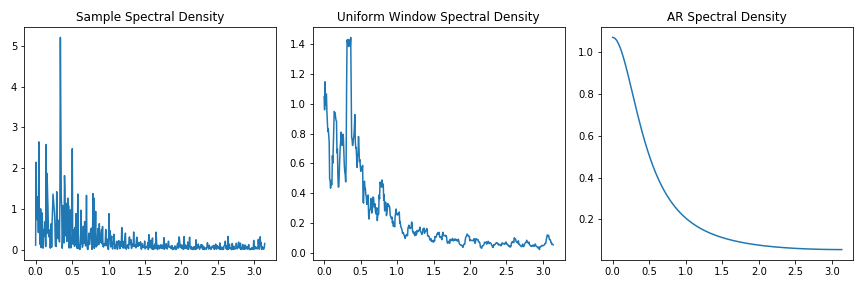
\includegraphics[width=\textwidth]{q3-fig}
\caption{}
\label{q3-fig}
\end{figure}
\end{proof}


\begin{prob}
Consider
\begin{align*}
	x_t &= y_{1t} - y_{1,t-1} \\ 
	z_t &= \frac{1}{3}(y_{1,t-1} + y_{1t} + y_{1,t+1}). 
\end{align*}
Repeat exercise 3 for $x_t$ and $z_t$. Compare the spectral densities of $x_t$, $z_t$, and $y_{1t}$. 
\end{prob}

\begin{proof}
The following code applies the first difference filter $b(L) = 1-L$ to $y_{1t}$ to generate $x_t$ and applies the moving average filter $h(L)=(L + 1 + L^{-1})/3$ to $y_{1t}$ to generate $z_t$. Then the function calls to \mintinline{python3}{sample_sdf},  \mintinline{python3}{unif_window}, and \mintinline{python3}{ar_sdf} used to generate estimates of the spectral densities of the $x_t$ and $z_t$ processes. 


\begin{python3code}
# First difference and moving average (lag 3) filter 
xt = np.diff(y1)
zt = np.convolve(np.ones(3)/3, y1, mode='valid')

# Sample SDFs
w_xt, f_xt = sample_sdf(xt)
w_zt, f_zt = sample_sdf(zt)

# Uniform lag window SDFs
w_xt_unif, f_xt_unif = unif_window(xt)
w_zt_unif, f_zt_unif = unif_window(zt)

# Sample SDFs
w_xt, f_xt = sample_sdf(xt)
w_zt, f_zt = sample_sdf(zt)

# Uniform lag window SDFs
f_xt_unif = unif_window(f_xt)
f_zt_unif = unif_window(f_zt)

# Autoregressive SDF estimation 
xt_freq, ar_sdf_xt = ar_sdf(xt)
zt_freq, ar_sdf_zt = ar_sdf(zt)

# Plot results
plt.figure(figsize=(12,4))

plt.subplot(131)
plt.plot(w_xt, f_xt, label='$x_t$')
plt.plot(w_zt, f_zt, label='$z_t$')
plt.legend()
plt.title('Sample Spectral Densities')

plt.subplot(132)
plt.plot(w_xt, f_xt_unif[1:], label='$x_t$')
plt.plot(w_zt, f_zt_unif[1:], label='$z_t$')
plt.title('Uniform Window Spectral Densities')

plt.subplot(133)
plt.plot(xt_freq, ar_sdf_xt, label='$x_t$')
plt.plot(zt_freq, ar_sdf_zt, label='$z_t$')
plt.title('Implied AR Spectral Densities')

plt.tight_layout()
plt.show()
\end{python3code}

Figure \ref{q4-fig} shows estimated spectral density functions for the $x_t$ and $z_t$ processes. Consider first the $x_t$ process. Since the spectrum of $x_t$ is related to the spectrum of $y_t$ by 
\[
	f_x(\omega) = b(e^{-i\omega})b(e^{i\omega}) f_y(\omega), 
\]
we analyze the function
\[
	b(e^{-i\omega})b(e^{i\omega}) = 2 - 2 \cos \omega,
\]
In the space $L_2[0,\pi]$, this function attains a maximum of 4 at $\omega=\pi$ and a minimum of 0 at $\omega=0$, and so this filter has the effect of emphasizing the high-frequency components of $y_{1t}$ and removing components at low frequencies. But from Problem 3 we know that $y_{1t}$ is primarily composed of low frequency components as confirmed by all three sample spectral density functions in Figure \ref{q3-fig}. It follows that all estimated sample spectral density function of $x_t$ are all mostly flat, increasing in value with $\omega$. As before, the estimates become smoother as the consistency of the estimators increases, which can be seen by observing the top, middle, then bottom graphs. 
\par
Consider now the $z_t$ process. Similarly, to understand the affect of this filter on the $y_{1t}$ process, we analyze the function
\[
	h(e^{-i\omega}) h(e^{i\omega}) = \frac{1}{3} (1+ e^{-i\omega} + e^{i\omega})\frac{1}{3} (1+ e^{i\omega} + e^{-i\omega}) = \frac{1}{9} (2 \cos \omega + 1)^2.
\]
In the space $L_2[0,\pi]$, this function attains a maximum of 1 at frequency $\omega=0$, monotonically decreasing to a minimum of 0 at frequency $\omega = 2 \pi/3$. This filter therefore accentuates components at frequency 0 and removes components at frequency $2 \pi/3$. The effect of including the $y_{1,t+1}$ term leads the $z_t$ process. This effect is most clearly observed by comparing the autoregressive spectral density estimates. It should be noted however that it is difficult to decipher this impact by comparing only the sample spectral density estimate and uniform window spectral density estimate in the first and second graphs in Figure \ref{q3-fig} and Figure \ref{q4-fig}, respectively. 

\begin{figure}
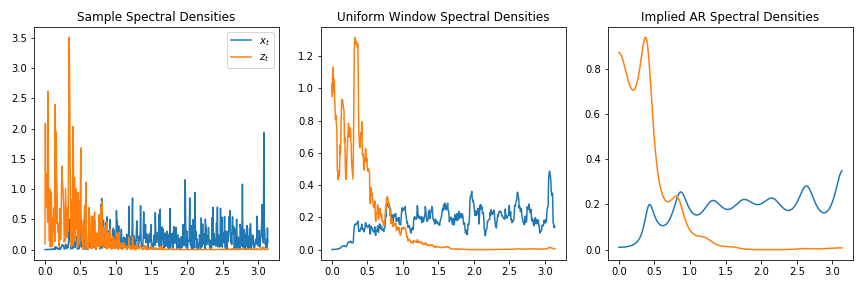
\includegraphics[width=\textwidth]{q4-fig}
\caption{}
\label{q4-fig}
\end{figure}
\end{proof}



\end{document}
